% !TEX root = ../main.tex
% Chapter: Discussion
\chapter{Discussion}
\label{ch:discussion}

% Booklet brief: begin with a 1--2 sentence summary, interpret rather than repeat Results,
% compare objectively with literature, identify failures and limitations, and propose
% improvements. The working draft deliberately shows both control routes. Before submission,
% exactly one route must be enabled in main.tex.
% Target after the final whole-document cut: approximately 1,750 words including ethics and
% future work. Percentages and percentage points follow the convention used in Results.

\section{Principal findings and their meaning}

This study implemented geometry-aware Mean Teacher training for pulmonary airway segmentation
and tested whether unlabelled CT changed recovery of the airway tree rather than only voxel
overlap.

\ifshowcurrentcontrol
\begin{currentcontrolroute}
The fitted Mean Teacher recovered more thin and deep airway structure on validation and held-out
data while its Dice score remained broadly unchanged, but the unpaired training runs restrict
this to a fitted-checkpoint comparison.

Against the current configuration-matched comparator, validation TLD and BD increased by
1.96 and 3.62 percentage points, respectively, whereas Dice decreased by 0.39 points. The
held-out ATM'22 cohort showed differences of similar size (TLD $+1.81$, BD $+3.79$ and Dice
$-0.09$ points). This reproducibility across patients and cohorts suggests that the two fitted
models occupy different operating points, but it does not establish a training-method effect:
their output heads and stochastic training trajectories were independently realised.
\end{currentcontrolroute}
\fi

\ifshowpairedcontrol
\begin{pairedcontrolroute}
Across the completed pairs, Mean Teacher \pending[: increased/did not consistently increase]
thin and deep airway recovery while Dice \pending[: remained stable/changed]; this supports
\pending[: a repeatable training-method effect/a run-specific fitted-model difference].

Across \pending[: number] complete seed pairs, Mean Teacher changed TLD by \pending and BD by
\pending percentage points, with effects in the same direction in \pending and \pending pairs;
Dice changed by \pending points. Because each eligible pair shared its complete initial state and
stochastic schedule, this estimates a fold-0 training-method effect rather than a difference
between two selected checkpoints. It remains conditional on one labelled split and the completed
pairs available by the pre-specified deadline.
\end{pairedcontrolroute}
\fi

The useful result is therefore the emph{shape} of the change, not a claim that the model became
uniformly better. The calibre, branch-depth and error-type analyses together ask whether the
consistency term changed where the network committed foreground and what it sacrificed to do so.

\ifshowcurrentcontrol
\begin{currentcontrolroute}
On validation, the TLD difference was 8.10 points in one-to-two-voxel airways, compared with
1.09 points at three to four voxels and no significant difference above four voxels. After
weighting by each band's share of the reference centreline, the one-to-two-voxel class supplied
approximately 65\% of the total TLD difference and the three-to-four-voxel class supplied the
remainder. Independently, the difference was negligible through branch depths 0--3 and rose to
2.83 points in the pooled $8+$ tail. BD followed the same depth profile, suggesting that reference
branches crossed the 80\% detection criterion rather than only acquiring isolated foreground
voxels. Agreement between the two axes localises the fitted-model difference to peripheral
reference structure, but does not distinguish anatomically valid extension from thin-branch
over-segmentation.
\end{currentcontrolroute}
\fi

\ifshowpairedcontrol
\begin{pairedcontrolroute}
Across complete pairs, the mean TLD effect was \pending in one-to-two-voxel airways and \pending
above four voxels. It was \pending through branch depths 0--3 and \pending in the pooled distal
tail, with the peripheral pattern present in \pending[: number] of \pending[: number] pairs.
Agreement between calibre and depth would support a repeatable peripheral redistribution;
disagreement would preclude a consistent localisation claim.
\end{pairedcontrolroute}
\fi

Airway-specific work has likewise identified foreground imbalance, discontinuity and peripheral
branch loss as related but distinct problems~\cite{qin2019airwaynet,zheng2021gradient,
yu2022break,Nan2024FANN}. The present analysis adds localisation along two measured anatomical
coordinates, while the selected control route determines whether that pattern belongs only to
two fitted models or generalises across training runs.

The apparent disagreement between Dice and tree recovery follows directly from airway geometry.
The one-to-two-voxel class contains 15.65\% of annotated centreline length but only 3.31\% of
airway volume. The same imbalance appears topologically: depths 0--3 contain 66.2\% of annotated
volume but only 12.2\% of centreline length. A volume-weighted score can therefore remain almost
fixed while a length-weighted score changes in the peripheral 87.8\% of the tree
~\cite{dice1945association,zheng2021gradient,shit2021cldice,zhang2023atm22}.

\ifshowcurrentcontrol
\begin{currentcontrolroute}
The error decomposition makes the exchange more specific. In one-to-two-voxel airways, the
8.10-point TLD difference was almost twice the 4.54-point voxel-recall difference, while precision
within predictions assigned to that class fell by 2.29 points. Above two voxels, voxel recall
fell while TLD was retained and voxel precision increased. This is a redistribution towards
centreline reach with fewer retained voxels elsewhere; it is not evidence that anatomical wall
thickness improved. Higher TLD is also insufficient by itself: a dilated or false-positive
extension that overlaps the reference centreline can raise coverage while creating an invalid
route. The fitted model therefore moved towards peripheral completeness at a bounded thin-branch
precision cost, rather than improving every part of the mask.

Whole-tree surfaces remain difficult to compare because most prediction voxels are shared.
Figure~\ref{fig:supp-qualitative} therefore traces one change across three scales. ATM~087 was
selected before rendering as the largest patient-level paired TLD gain, making it an illustrative
mechanistic best case rather than a representative patient. Panel A localises the change on the
whole tree; Panel B isolates the same region in 3-D; and Panel C places the selected component on
the underlying CT and reference annotation. The component was selected automatically before
visual inspection as the largest connected, thin and elongated annotated volume present only
under Soft-clDice. It spans 12.3~mm along its long axis, contains 83 newly correct foreground
voxels and accounts for 18 Soft-clDice-only reference-centreline voxels. Thus the patient-level
TLD improvement can, in this example, be spatially attributed partly to a coherent
reference-supported addition rather than merely to a diffuse change in segmentation overlap.
Preserving such distal paths is relevant to airway morphometry and navigation
~\cite{Wang2023qct,Dhillon2017PeripheralBronchoscopy,HammadAltaq2023robotic}, but this example does
not show that Soft-clDice generally restores distal branches, nor does it establish downstream
connectivity, bronchoscopic traversability or clinical benefit.
\end{currentcontrolroute}

\begin{figure}[p]
  \centering
  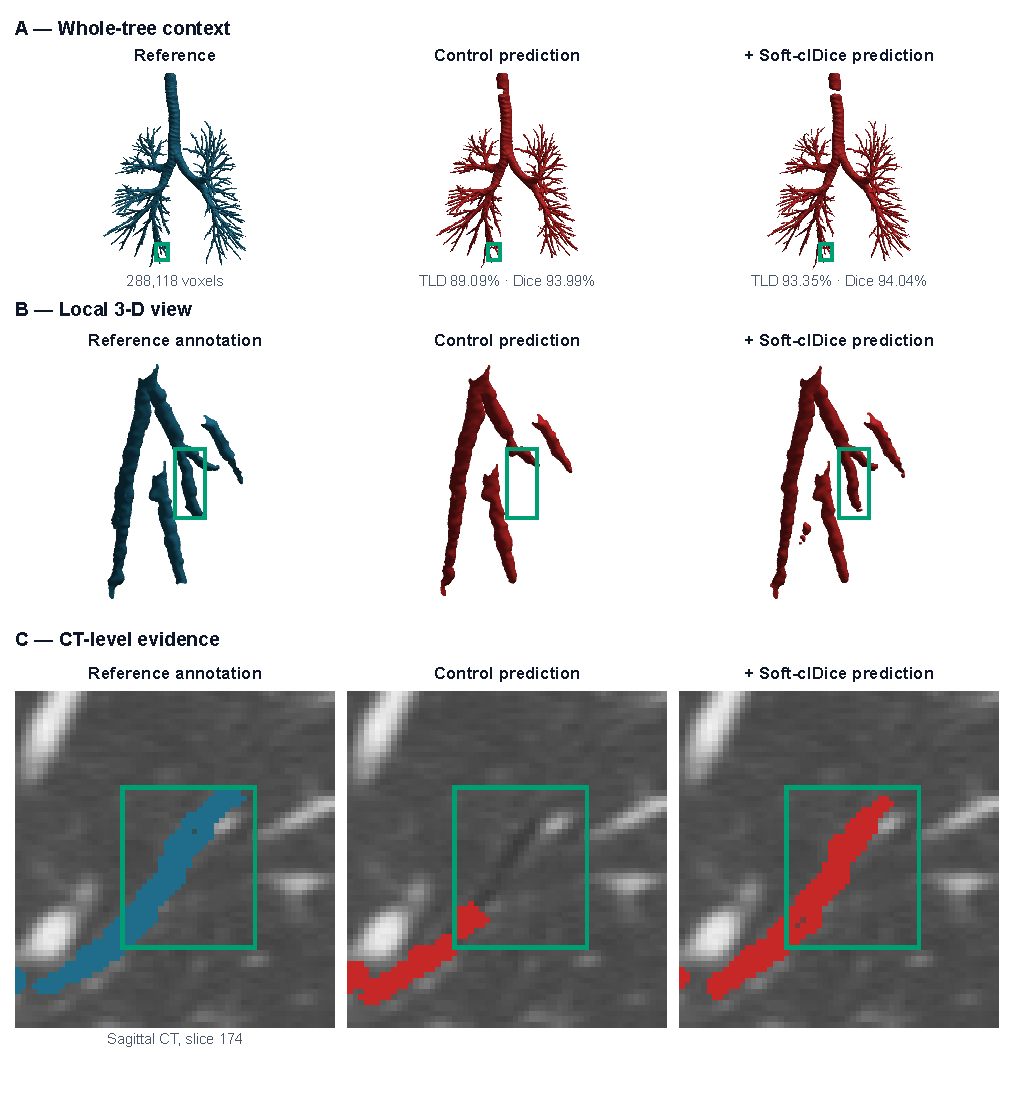
\includegraphics[width=\linewidth,height=0.79\textheight,keepaspectratio]{Figures/pdf/discussion/qualitative_plate_val_087.pdf}
  \caption[Multiscale localisation of a reference-supported addition]{Illustrative mechanistic
  best case, not cohort-level evidence. ATM~087 was selected before rendering as the largest
  patient-level paired TLD gain ($89.09\%$ to $93.35\%$; $+4.26$ percentage points). A gives
  whole-tree context and boxes the region; B enlarges the same 3-D segment; C shows its location on
  sagittal CT. Each row has the same order: reference annotation, control prediction and
  Soft-clDice prediction. Blue denotes the reference mask, red the model predictions, and green
  boxes identify the same region rather than an additional segmentation class. The automatically
  selected component contains 83 foreground and 18 centreline voxels and spans 12.3~mm. It
  spatially explains part of this patient's TLD difference but does not establish generally
  recovered anatomy or clinical utility.}
  \label{fig:supp-qualitative}
\end{figure}
\fi

\ifshowpairedcontrol
\begin{pairedcontrolroute}
Across complete pairs, voxel precision changed by \pending overall and by \pending in the
one-to-two-voxel class, while centreline precision changed by \pending. These results support
\pending[: a repeatable shift towards peripheral completeness/a less stable recall--precision
trade-off], rather than uniform improvement.
\end{pairedcontrolroute}
\fi

\section{Why the change localised to thin and deep airways}

The loss supplies the first part of a mechanistic explanation. Voxelwise MSE in
Equation~\eqref{eq:lmse} counts every cross-sectional voxel, so wide proximal structures can
contribute more disagreement than a narrow branch of the same length. By contrast, the
directional terms of Equation~\eqref{eq:tterms} normalise against soft-skeleton mass. Soft-clDice
has improved connectivity in tubular segmentation~\cite{shit2021cldice}; related semi-supervised
airway and vessel work likewise replaces plain voxel agreement with specialised or cross-geometry
representations~\cite{gu2023featurespecialisation,zhu2024crossgeometry}. The claim here is narrower
than the topological guarantee proved for binary masks: finite soft morphology on probability maps
neither enforces one connected airway tree nor establishes that a predicted branch is
anatomically correct.

The implementation introduces a more specific effect. As Figure~\ref{fig:soft-skeleton-iteration}
shows, a structure at most two voxels across is annihilated by the first cross erosion. Its opening
is then zero and the depth-zero residual equals the entire probability structure, rather than an
ideal one-voxel centreline. In the implementation-matched probe, the one-to-two-voxel class
formed 9.47\% of sampled teacher foreground but 28.69\% of teacher soft-skeleton mass: a
threefold relative representation. The apparent defect therefore does not suppress the thinnest
tree. It acts as an accidental thin-structure weighting, summarised in
Figure~\ref{fig:discussion-mechanism}.

\begin{figure}[htbp]
  \centering
  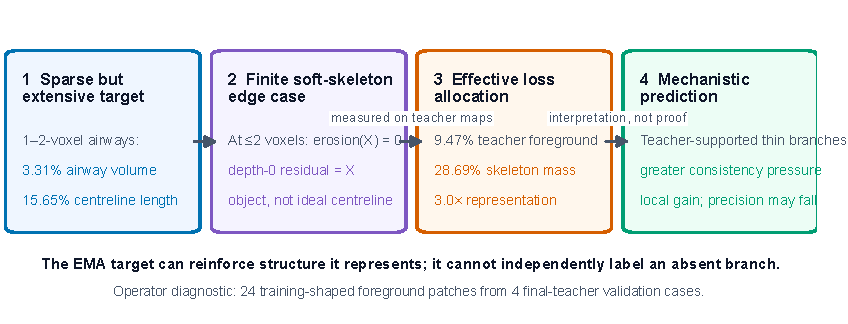
\includegraphics[width=\linewidth]{Figures/pdf/discussion/mean_teacher_mechanism.pdf}
  \caption[Mechanistic account of the thin-airway effect]{Implementation-matched account of how
  thin airways acquire leverage in the consistency loss. The target census uses the 20-case
  validation cohort. The loss-allocation diagnostic uses 24 training-shaped, foreground-centred
  patches sampled from four final EMA-teacher probability maps. Solid arrows join definitions or
  measurements; the dashed arrow is a mechanistic interpretation, not causal proof. The predicted
  localisation is tested independently by the calibre and depth results in
  Figures~\ref{fig:calibre-delta} and~\ref{fig:depth-recovery}.}
  \label{fig:discussion-mechanism}
\end{figure}

The same probe explains why twofold upsampling is not an automatic repair. Upsampling reduced
the fraction of teacher foreground annihilated by one erosion from 34.03\% to 20.39\% and reduced
total skeleton mass from 8.78\% to 3.07\% of foreground, so it produced a geometrically thinner
skeleton. However, the thinnest class still received 25.89\% of skeleton mass, compared with
28.69\% at native resolution, while a checkpointed consistency pass increased from approximately
0.16 to 3.10 seconds. It changes the skeleton's magnitude far more than the relative allocation
that drives the normalised sensitivity term. A full upsampled training arm could therefore spend
substantial compute while also weakening the accidental weighting associated with the primary
effect; geometric correctness alone does not predict a better fitted model.

\ifshowcurrentcontrol
\begin{currentcontrolroute}
The predicted signature is present: this class produced the largest fitted-model TLD difference
in all 20 validation cases and approximately 65\% of the aggregate difference. The concordance
between an implementation-derived prediction and a separately measured outcome supports the
weighting mechanism, although the post-hoc probe and unpaired checkpoints do not identify it
causally.
\end{currentcontrolroute}
\fi

\ifshowpairedcontrol
\begin{pairedcontrolroute}
The paired effect was \pending[: largest/not consistently largest] in this class, which
\pending[: supports/does not support] thin-structure weighting as a repeatable mechanism.
\end{pairedcontrolroute}
\fi

Neither route shows that differentiable skeletonisation preserved topology for its intended
mathematical reason. This distinction is important because
recent airway methods obtain structural gains through different mechanisms, including
connectivity-aware learning, feature specialisation and multi-task topology enhancement
~\cite{qin2019airwaynet,gu2023featurespecialisation,yang2024topoenhance}.

Calibre does not, however, explain the entire spatial pattern. Across the reference centreline,
branch depth and calibre were only moderately correlated ($\rho=-0.48$): 94.3\% of the
one-to-two-voxel centreline lay at depth~5 or deeper, but 81.0\% of the depth-$\geq5$ centreline
was wider than two voxels. Thus ``thin'' usually means peripheral, but ``peripheral'' does not
mean only the thinnest class.

\ifshowcurrentcontrol
\begin{currentcontrolroute}
Descriptively, the fitted TLD difference still increased with depth within the fixed
one-to-two- and three-to-four-voxel bands ($\rho=0.78$ and $0.98$). The 110-label supervised
reference showed the same depth-graded shape at smaller magnitude through depths 4--7. The
location is therefore a general signature of improving peripheral recovery, while the
soft-skeleton weighting plausibly helps set its magnitude.
\end{currentcontrolroute}
\fi

\ifshowpairedcontrol
\begin{pairedcontrolroute}
Within fixed calibre bands, the across-pair TLD effect changed with depth by \pending. A retained
depth trend would support a spatial effect beyond calibre; its absence would restrict the
mechanistic account to thin-structure weighting.
\end{pairedcontrolroute}
\fi

This remaining depth association is plausibly produced by the interaction between the target and
the data. Peripheral lumina approach the acquisition resolution, so partial-volume effects and
weak contrast make their predictions less stable under intensity perturbation
~\cite{montaudon2007,GarciaUceda2021AirwayCNN}. EMA averaging supplies a temporally smoother target
~\cite{tarvainen2017mean,laine2017temporal,yu2019uamt}; consistency can therefore discourage the
student from intermittently dropping a weak branch that the teacher already represents. It does
not encode branch depth explicitly, so this remains an evidence-consistent explanation rather
than a learned anatomical-depth mechanism.

The consistency-weight sweep explains why gains in tree recovery are accompanied by losses
elsewhere. Increasing $w_{\max}$ from 0.03 to 0.30 monotonically increased TLD and BD, but topology
precision fell from 92.27\% to 86.69\% and the corresponding evaluation clDice fell from 92.48\%
to 90.61\% (Table~\ref{tab:weight-sensitivity}). A larger weight therefore made the network commit
to more reference centreline while accepting more unsupported predicted centreline. This is an
operating-point curve, not monotonic improvement, and no turning point was bracketed.

\ifshowcurrentcontrol
\begin{currentcontrolroute}
Only $w_{\max}=0.10$ has five-fold, held-out and out-of-distribution evaluation.
\end{currentcontrolroute}
\fi

\ifshowpairedcontrol
\begin{pairedcontrolroute}
The seeded programme fixes $w_{\max}=0.10$; the other weights remain single-run sensitivity
points and do not estimate variation in the weight response.
\end{pairedcontrolroute}
\fi

\ifshowcurrentcontrol
\begin{currentcontrolroute}
The voxel-MSE arm at $w_{\max}=0.30$ remained close to the configuration comparator. This is
consistent with the proposed normalisation account: Equation~\eqref{eq:lmse} averages disagreement
over the patch, whereas Equation~\eqref{eq:tterms} allocates it through skeleton mass. Similar
concerns motivate geometry- and distance-consistency methods for tubular targets
~\cite{gu2023featurespecialisation,zhu2024crossgeometry,zhao2025vesselselftraining}. It is not
controlled proof that soft-clDice is superior, because the objectives were not weight-matched and
their gradient scales differ.
\end{currentcontrolroute}
\fi

\ifshowpairedcontrol
\begin{pairedcontrolroute}
The existing voxel-MSE result is not part of the seeded treatment contrast: it is one run at
$w_{\max}=0.30$ without an identical-state MSE--control pair. It therefore provides descriptive
evidence about that fitted objective, not an across-seed comparison with soft-clDice.
\end{pairedcontrolroute}
\fi

A matched plain and foreground--background-balanced MSE comparison is needed before attributing
the result specifically to centreline geometry.

The mechanism also explains why stronger consistency eventually loses precision. The target is
an EMA model, not the reference annotation. If a teacher extension is stable but anatomically
wrong, increasing its weight makes the student more consistent with that error; this is analogous
to confirmation bias in pseudo-label learning~\cite{arazo2020confirmation}. Conversely, Mean
Teacher cannot provide independent positive evidence for a branch wholly absent from the teacher.
EMA averaging can stabilise a represented branch under perturbation
~\cite{tarvainen2017mean,laine2017temporal,yu2019uamt}, but teacher and student errors remain
correlated. Supervised gradients may still let the student exceed its teacher, so this is an
information constraint rather than an absolute ceiling.

That constraint is stronger in the implemented experiment because ordinary spatial augmentation
was shared between the two streams; only the additional intensity scale, shift and noise of
Equation~\eqref{eq:perturbation} separated them. The unlabelled signal therefore tests whether an
existing structure survives photometric perturbation, not whether two independent anatomical
views discover the same branch. This makes consolidation of weak teacher-supported evidence a
more likely explanation than anatomical discovery. Feature-specialised peers and task-level
cross-geometry consistency are credible alternatives precisely because they create more distinct
representations~\cite{gu2023featurespecialisation,zhu2024crossgeometry}.

\section{Robustness and relation to prior work}

\ifshowcurrentcontrol
\begin{currentcontrolroute}
Five-fold ensembling improved the balance between volumetric and topology-aware metrics and
removed the severe connected-component failure observed in one fold. It is the preferred
absolute deployment estimate, but the absence of a five-fold control means that it cannot be
used as a second treatment contrast. Similarly, the supervised model trained from a 110-case
pool supplies label-scale context rather than a ceiling or causal comparator: it differs in
training cases and pipeline. The fact that several Mean Teacher models exceed it in TLD while
not uniformly exceeding Dice or precision reinforces the need to report complementary measures,
as adopted by ATM'22~\cite{zhang2023atm22}.
\end{currentcontrolroute}
\fi

\ifshowcurrentcontrol
\begin{currentcontrolroute}
The fitted-model TLD and BD ordering persisted on held-out ATM'22 data and was attenuated on
AeroPath. This is evidence of retrospective robustness rather than clinical generalisability.
\end{currentcontrolroute}
\fi

\ifshowpairedcontrol
\begin{pairedcontrolroute}
The mean paired effect changed from \pending on validation to \pending on held-out ATM'22 and
\pending on AeroPath, retaining its direction in \pending and \pending complete pairs. This
provides \pending[: cross-cohort support/no stable external support] for the fold-0 effect.
\end{pairedcontrolroute}
\fi

AeroPath was designed to include pathology that challenges airway segmentation
~\cite{stoverud2023aeropath}, but acquisition spacing, annotation policy and case mix differ, so
absolute voxel-calibre bands are not directly transferable. Published semi-supervised airway
studies also use different labelled fractions, cohorts and baselines
~\cite{gu2023featurespecialisation,zhu2024crossgeometry}; numerical ranking against them would
therefore confound method with data and evaluation. The more useful comparison is conceptual:
all treat peripheral airway structure as a problem that conventional voxel consistency does not
fully represent, while this study additionally exposes how sensitive that conclusion is to the
choice of control.

\section{Limitations and improvements}

\ifshowcurrentcontrol
\begin{currentcontrolroute}
The dominant limitation is unmeasured training variation. Patient-paired tests and bootstrap
intervals quantify variation across evaluation cases conditional on two checkpoints; they do not
include variation from initialisation, data order, augmentation, GPU execution or labelled fold.
The present comparison should therefore be called a configuration contrast. Identical-state,
seed-paired control--Mean Teacher continuations are the direct improvement.
\end{currentcontrolroute}
\fi

\ifshowpairedcontrol
\begin{pairedcontrolroute}
Seed pairing measures training variation only for fold~0. It does not cover different labelled
splits, hardware or unpaired failures, and \pending[: number] completed pairs provide limited
precision for an across-seed effect. Replicating complete pairs on the remaining folds is the
direct improvement.
\end{pairedcontrolroute}
\fi

Each primary fold trained with 16 labelled patients, so augmentation increases the number of
views but not anatomical diversity. The held-out ATM'22 cohort is also not pristine confirmation:
historical development models had accessed it before the present comparison was frozen. AeroPath
adds a second case distribution, but neither cohort establishes performance across scanners,
institutions or demographic groups. Multicentre evaluation with metadata-defined subgroups is
required before making a population-level claim.

The unlabelled-pool experiment also did not isolate data quantity. Expanding the pool from 90 to
240 scans under 125{,}000 unlabelled draws reduced mean exposure from 1{,}388.9 to 520.8 draws per
scan. Increasing the number of unlabelled patches then changed compute as well as exposure. The
observed differences therefore cannot show whether the additional 150 scans lacked useful
information; a smaller-pool arm with matched exposure is the missing comparison.

Measurement introduces further uncertainty. TLD and BD depend on skeletonisation, junction
handling and an in-house branch parser that has synthetic tests but no golden parity test against
the official ATM'22 evaluator. Depth is a graph-derived branching order rather than Weibel
generation~\cite{weibel1963morphometry,tschirren2005airway,palagyi2006airway}. Centreline geometry is used both in the
training objective and in several outcomes, so Dice and precision remain necessary independent
checks. Reference annotations are themselves limited by CT resolution and annotation policy in
the distal tree; an additional plausible branch cannot be assumed correct simply because it
looks anatomically continuous. Finally, connected-component filtering can delete a genuine
subtree after one proximal break. Treating native output as primary and connected output as a
declared sensitivity makes that failure visible rather than averaging it away.

\section{Ethical considerations}

Engineering guidance places honesty, accuracy, public safety and communication of uncertainty at
the centre of professional practice~\cite{engineeringcouncil2026ethics}. For this study,
scientific integrity requires disclosure that a sampler fault invalidated an early arm and that
negative ablations were retained.

\ifshowcurrentcontrol
\begin{currentcontrolroute}
The configuration comparator is not a seeded causal control, and the current checkpoints cannot
be reproduced bit-for-bit. Integrity therefore rests on disclosing those limits rather than
hiding them behind patient-paired statistics.
\end{currentcontrolroute}
\fi

\ifshowpairedcontrol
\begin{pairedcontrolroute}
The prospective pairs pre-specify complete initial states, seeds, eligibility and checkpoint
policy. Integrity requires reporting incomplete pairs and deviations as well as successful runs;
pairing does not remove uncertainty from labelled fold, hardware or scoring provenance.
\end{pairedcontrolroute}
\fi

Configurations, code versions and machine-readable outputs improve reproducibility. Thresholds,
checkpoints and post-processing should not be selected after inspecting the desired outcome. This
follows Imperial's principles of integrity, proportional risk, beneficence and non-maleficence
~\cite{imperial2025ethicalframework}.

No new participant or animal was recruited, scanned or exposed to an intervention. ATM'22 and
AeroPath are public secondary datasets whose publishers describe their data provenance
~\cite{zhang2023atm22,stoverud2023aeropath}. Nevertheless, public availability does not remove
duties of confidentiality, licence compliance and purpose-limited use. Case examples should
remain anonymised, and any redistribution must follow each dataset's licence or access agreement.
The people represented in the training data are also not necessarily those who would bear deployment errors, so aggregate
performance cannot establish distributive fairness.

The direction of error matters clinically. A false-negative branch could hide a possible route,
whereas a confident false-positive branch could suggest a bronchoscopic path that does not exist
~\cite{Dhillon2017PeripheralBronchoscopy,HammadAltaq2023robotic}. A visually plausible tree may
encourage automation bias, particularly when connected-component processing converts a broken
prediction into a clean-looking but incomplete result. WHO guidance consequently emphasises
human oversight, accountability, inclusiveness and continuing evaluation for health AI
~\cite{who2021aiguidance}; software used for clinical decisions would also require an appropriate
medical-device evidence and governance pathway~\cite{mhra2025aimd}. The present models should
therefore remain research tools unless prospectively validated with clinician oversight,
failure warnings and application-specific acceptance criteria.

Computational cost is also an ethical trade-off. Retained logs account for at least 356 GPU-hours,
excluding failed, missing and queued jobs, so this is a lower bound rather than metered total
energy. Carbon estimates depend on accelerator power, host memory, data-centre efficiency and grid
intensity~\cite{lannelongue2021green}. Pre-specifying a limited number of paired runs, reusing
saved predictions for secondary analyses and publishing negative results reduce avoidable
repetition; the final
report should replace this floor with the scheduler-derived total.

\section{Future work}

\ifshowcurrentcontrol
\begin{currentcontrolroute}
The first priority is to complete identical-state control--Mean Teacher seed pairs and then
replicate them across labelled folds. Until then, additional performance tuning cannot repair the
main inferential weakness.
\end{currentcontrolroute}
\fi

\ifshowpairedcontrol
\begin{pairedcontrolroute}
With fold-0 seed variation estimated, the first priority is complete-pair replication across
labelled folds and external cohorts. This tests whether the effect survives a different labelled
sample rather than only a different training trajectory.
\end{pairedcontrolroute}
\fi

The next ablations should separate mechanisms rather than add an undirected sweep. First, plain
and foreground--background-balanced MSE must be compared at the same $w_{\max}$ and initial state
as soft-clDice. Extending the consistency-weight range is useful only until it brackets a turning
point or collapse; replication at a selected weight is then more informative than adding rungs.
Second, changing the soft-skeleton iteration depth from the reported $K=10$ can test the finite
representation of wider structures, but it cannot remove the depth-zero edge case that weights
one-to-two-voxel branches. It is therefore a secondary ablation, not a direct test of the primary
mechanism. A direct test would alter the iteration-zero contribution, or compare native and
upsampled skeletonisation at a shared initial state, then ask whether the thin-band effect weakens
as predicted. The existing twofold probe shows that upsampling repairs the morphology at an
approximately twentyfold per-pass time cost while leaving relative thin-band allocation similar;
a full arm is justified only if that mechanistic question outweighs seed replication. A 90-scan
arm with unlabelled exposure matched to the 240-scan arm would separately estimate the value of
pool size.

The central information constraint requires a different experiment. Replacing the EMA target
temporarily with a more fully supervised teacher would distinguish teacher capacity from the
consistency mechanism, although it would be a diagnostic that imports label information rather
than a deployable semi-supervised method. Independently initialised peers, or a segmentation and
distance-transform dual head with cross-geometry and Hausdorff consistency, could then introduce
genuinely different representations~\cite{zhu2024crossgeometry}. A fully supervised 260-label
model would strengthen label-scale context but would still not replace the matched continuation
control. Finally, metric parity testing and prospective multicentre, clinician-facing evaluation
are prerequisites for anatomical or clinical claims.
